\documentclass[aspectratio=169,11pt]{beamer}
\usepackage[utf8]{inputenc}
\usepackage[T1]{fontenc}
\usepackage{amsmath,amssymb}
\usepackage{graphicx}
\usepackage{booktabs}
\usepackage{tikz}
\usetikzlibrary{arrows.meta,positioning,shapes.geometric,backgrounds,fit}
\graphicspath{{../figures/}}

% ---- clean flat look (no external theme dependency) -------------------------------
\usetheme{default}
\usecolortheme{seahorse}
\setbeamertemplate{navigation symbols}{}
\definecolor{brandblue}{RGB}{26,115,232}
\definecolor{brandgray}{RGB}{95,99,104}
\definecolor{brandred}{RGB}{217,48,37}
\definecolor{brandgreen}{RGB}{24,128,56}
\definecolor{inkdark}{RGB}{32,33,36}
\setbeamercolor{frametitle}{fg=brandblue,bg=white}
\setbeamercolor{title}{fg=brandblue}
\setbeamercolor{structure}{fg=brandblue}
\setbeamerfont{frametitle}{series=\bfseries}
\setbeamertemplate{frametitle}{\vspace{0.3em}\insertframetitle\vspace{-0.2em}}
\setbeamertemplate{footline}[frame number]
\setbeamercovered{transparent}

% section divider frames
\AtBeginSection[]{%
  \begin{frame}[plain]\centering\vfill
    {\usebeamerfont{title}\color{brandblue}\bfseries\insertsectionhead}\vfill
  \end{frame}}

\newcommand{\kj}{\,kJ/mol}
\newcommand{\arw}{$\rightarrow$}

\title{\bfseries A Unified First-Principles Pipeline for\\Metabolic Reaction Free Energies}
\subtitle{Automatic QM routing over the ModelSEED reaction space}
\author{Ray Zhu}
\date{\today}

\begin{document}

% ---- 1. TITLE ---------------------------------------------------------------------
{\setbeamertemplate{footline}{}
\begin{frame}[plain]
  \titlepage
  \begin{center}\small\color{brandgray}
  UMA machine-learned QM \;$\cdot$\; pH-0 anion routing \;$\cdot$\; self-gating \;$\cdot$\; calibrated UQ
  \end{center}
\end{frame}}

% ---- 2. THE PROBLEM ---------------------------------------------------------------
\begin{frame}{The problem: $\Delta_r G$ for the whole metabolic network}
  \begin{columns}[T]
    \begin{column}{0.56\textwidth}
      \begin{itemize}
        \item Thermodynamics gates flux: every FBA / TFA model needs $\Delta_r G^{\prime\circ}$.
        \item Group-contribution (GCM, dGPredictor) is fast \& accurate \emph{in-domain} \dots
        \item \dots but \textbf{refuses $\sim$42\% of ModelSEED} — mass/charge-imbalanced, novel groups, off-distribution.
        \item \textbf{QM is parameter-free} and covers that frontier — \emph{if} it can be made accurate and automatic.
      \end{itemize}
      \vspace{0.5em}
      \begin{block}{Goal}
        One pipeline, \textbf{no per-reaction tuning}, that scores any balanced reaction from structure alone.
      \end{block}
    \end{column}
    \begin{column}{0.42\textwidth}
      \centering
      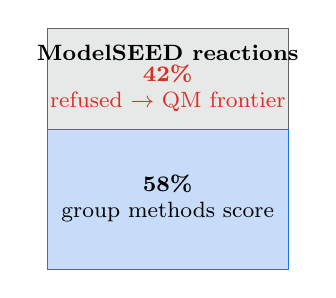
\begin{tikzpicture}[scale=0.9,every node/.style={font=\footnotesize}]
        \draw[fill=brandgray!15,draw=brandgray] (0,0) rectangle (3.4,3.4);
        \node at (1.7,3.05) {\bfseries ModelSEED reactions};
        \draw[fill=brandblue!25,draw=brandblue] (0,0) rectangle (3.4,1.97);
        \node[align=center] at (1.7,1.0) {\bfseries 58\%\\group methods score};
        \node[align=center,text=brandred] at (1.7,2.55) {\bfseries 42\%\\refused $\to$ QM frontier};
      \end{tikzpicture}
      \\[0.3em]{\scriptsize 20{,}802 balanced reactions are QM-runnable today (57$\times$ TECRDB).}
    \end{column}
  \end{columns}
\end{frame}

% ---- 3. WHY NAIVE QM FAILS --------------------------------------------------------
\begin{frame}{Why naive QM fails on metabolites}
  \begin{columns}[T]
    \begin{column}{0.58\textwidth}
    \textbf{Two failure modes, both large:}
    \begin{enumerate}
      \item \textbf{Anion-solvation catastrophe.} Implicit continuum mis-solvates each
      polyphosphate charge state by $\pm20$–$50\kj$, and the errors are \emph{sign-varying}
      — they do \textbf{not} cancel in $\Delta_r G$.
      \item \textbf{Conformer noise} on huge, floppy substrates (sugar-phosphates, cofactors):
      spectator backbone dominates the energy and drowns the reactive signal.
    \end{enumerate}
    \vspace{0.4em}
    \begin{itemize}
      \item Worst for the ML potential (UMA): formal anionic charge $+$ diffuse density $+$ non-local delocalisation.
      \item Baseline MAE \textbf{29\kj}; \emph{huge/floppy} class \textbf{45\kj}.
    \end{itemize}
    \end{column}
    \begin{column}{0.40\textwidth}
      \centering
      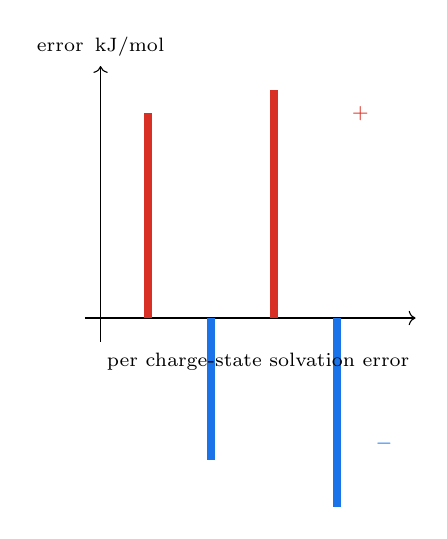
\begin{tikzpicture}[every node/.style={font=\scriptsize}]
        \draw[->] (0,-0.3) -- (0,3.2) node[above]{error \kj};
        \draw[->] (-0.2,0) -- (4.0,0);
        \foreach \x/\v/\c in {0.6/2.6/brandred, 1.4/-1.8/brandblue, 2.2/2.9/brandred, 3.0/-2.4/brandblue} {
          \draw[\c,line width=3pt] (\x,0) -- (\x,\v);
        }
        \node[align=center] at (2.0,-0.55){per charge-state solvation error};
        \node[text=brandred] at (3.3,2.6){$+$};
        \node[text=brandblue] at (3.6,-1.6){$-$};
      \end{tikzpicture}
      \\[0.2em]{\scriptsize Opposite signs $\Rightarrow$ scatter, not a subtractable bias.}
    \end{column}
  \end{columns}
\end{frame}

% ---- 4. THE PIPELINE (architecture) -----------------------------------------------
\begin{frame}{The idea: one self-routing pipeline}
  \centering
  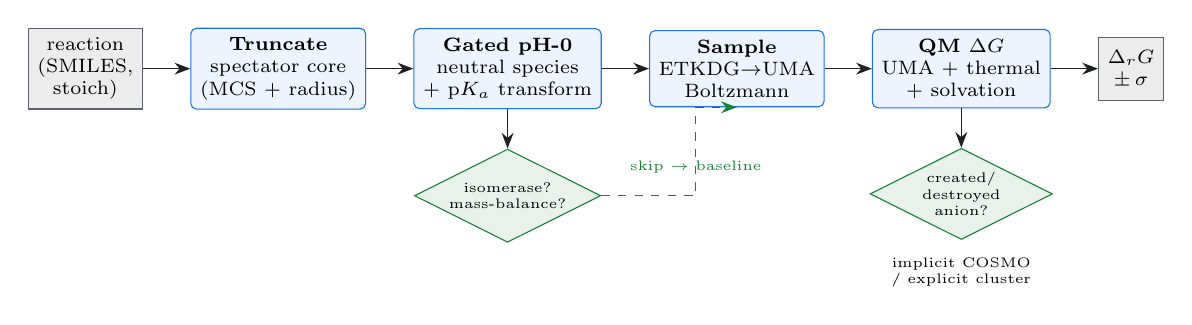
\begin{tikzpicture}[
      node distance=6mm,
      box/.style={rectangle,rounded corners=2pt,draw=brandblue,fill=brandblue!8,
                  minimum height=8mm,minimum width=20mm,align=center,font=\scriptsize},
      gate/.style={diamond,aspect=2,draw=brandgreen,fill=brandgreen!10,align=center,font=\tiny,inner sep=1pt},
      io/.style={rectangle,draw=brandgray,fill=brandgray!12,minimum height=8mm,align=center,font=\scriptsize},
      a/.style={-{Stealth[length=2mm]},draw=inkdark}]
    \node[io] (in) {reaction\\(SMILES,\\stoich)};
    \node[box,right=of in] (tr) {\textbf{Truncate}\\spectator core\\(MCS + radius)};
    \node[box,right=of tr] (ph0) {\textbf{Gated pH-0}\\neutral species\\$+$ p$K_a$ transform};
    \node[box,right=of ph0] (samp) {\textbf{Sample}\\ETKDG$\to$UMA\\Boltzmann};
    \node[box,right=of samp] (qm) {\textbf{QM $\Delta G$}\\UMA $+$ thermal\\$+$ solvation};
    \node[io,right=of qm] (out) {$\Delta_r G$\\$\pm\,\sigma$};
    \draw[a] (in)--(tr); \draw[a] (tr)--(ph0); \draw[a] (ph0)--(samp);
    \draw[a] (samp)--(qm); \draw[a] (qm)--(out);
    % gates under pH0
    \node[gate,below=5mm of ph0] (g1) {isomerase?\\mass-balance?};
    \draw[a] (ph0.south) -- (g1.north);
    \draw[a,dashed,brandgreen] (g1.east) -- ++(1.2,0) |- (samp.south) node[pos=0.25,below,font=\tiny,text=brandgreen]{skip $\to$ baseline};
    % solvation triage under qm
    \node[gate,below=5mm of qm] (g2) {created/\\destroyed\\anion?};
    \draw[a] (qm.south)--(g2.north);
    \node[font=\tiny,below=1mm of g2,align=center]{implicit COSMO\\ / explicit cluster};
  \end{tikzpicture}
  \vfill
  {\footnotesize Every stage is a \textbf{general heuristic} — chosen from structure, no reaction-id, no fitting to the benchmark.}
\end{frame}

% ---- 5. TRUNCATION ----------------------------------------------------------------
\begin{frame}{Stage 1 — Spectator truncation}
  \begin{columns}[T]
    \begin{column}{0.6\textwidth}
    \begin{itemize}
      \item Map the reaction, keep the \textbf{reactive core} (atoms that change bonding) $+$ a radius shell, cap open valences.
      \item Removes the conserved backbone \arw{} kills catastrophic cancellation \emph{and} its conformer noise.
      \item \textbf{Radius-sensitivity guard}: escalate the shell until $\Delta G$ is stable
      (good cut $|\Delta\Delta G|{=}1.3$; bad cut $27.7$ \arw{} rejected).
      \item \texttt{v2} global-map extends it to the 20\% multi-coefficient / unequal-side reactions.
    \end{itemize}
    \end{column}
    \begin{column}{0.38\textwidth}
      \begin{block}{Example}
        rxn03643 (glycosyl transfer)\\[0.3em]
        full molecule: $-10\kj$ error\\
        truncated core: \textbf{$+1.4\kj$}
      \end{block}
      {\scriptsize After pH-0, truncated $\approx$ full-molecule error — truncation mainly buys \emph{robustness} and speed.}
    \end{column}
  \end{columns}
\end{frame}

% ---- 6. pH-0 ----------------------------------------------------------------------
\begin{frame}{Stage 2 — pH-0 neutral-species routing \small(the accuracy breakthrough)}
  \textbf{Idea (Jinich 2014/18; Alberty transform):} don't compute the mis-solvated anion.
  Protonate \emph{every} anionic site to its \textbf{neutral} microspecies — UMA's comfortable
  regime — then bridge to pH 7 \emph{analytically} with textbook p$K_a$'s:
  \[
    \Delta_r G^{\prime}(\mathrm{pH\,7}) \;=\; \underbrace{\Delta_r G_{\mathrm{QM}}(\text{all-neutral})}_{\text{no formal charge}}
    \;+\; \sum_{\text{sites }i} s_i\, RT\ln\!\big(1+10^{\,\mathrm{pH}-\mathrm{p}K_{a,i}}\big),
    \quad s_i=\!\begin{cases}+1&\text{react}\\-1&\text{prod}\end{cases}
  \]
  \begin{columns}[T]
    \begin{column}{0.6\textwidth}
      \begin{itemize}
        \item No atom-mapper: matched spectator anions \textbf{cancel} analytically.
        \item Max-anion canonicalisation \arw{} protonation-source-independent.
        \item Exact Alberty form (not linear) — correct near \emph{and} above p$K_a$.
        \item Nothing fitted to the DB — p$K_a$'s are textbook.
      \end{itemize}
    \end{column}
    \begin{column}{0.38\textwidth}
      \begin{block}{Validated}
        rxn00695 (adenylyltransferase)\\ \quad $-96 \to \mathbf{+0.2}\kj$\\[0.2em]
        rxn10427 (adenylate kinase)\\ \quad $+61 \to \mathbf{+4.8}\kj$
      \end{block}
    \end{column}
  \end{columns}
\end{frame}

% ---- 7. SELF-GATING ---------------------------------------------------------------
\begin{frame}{Stage 2 makes itself safe: two structural gates}
  \begin{columns}[T]
    \begin{column}{0.5\textwidth}
      \textbf{Isomerase gate}
      \begin{itemize}\footnotesize
        \item If every reactant formula matches a product formula (a rearrangement), there is
        \emph{no} anion-solvation change to fix.
        \item pH-0 would only inject neutral-vs-anion noise \arw{} \textbf{skip}, use baseline.
      \end{itemize}
      \vspace{0.6em}
      \textbf{H-mass-balance guard}
      \begin{itemize}\footnotesize
        \item pH-0 fixes $n_{\mathrm{H^+}}{=}0$ (the transform carries all proton exchange).
        \item Only valid when re-protonation is H-balanced:
        \[ \textstyle\sum_i \nu_i\, H(\text{neutral}_i) = 0. \]
        \item Else refuse \arw{} baseline.
      \end{itemize}
    \end{column}
    \begin{column}{0.48\textwidth}
      \begin{alertblock}{The bug this caught}
        \footnotesize Net-proton reactions (NAD(P)/GSH \textbf{redox}, deamination) drop one
        proton when forced to $n_{\mathrm{H^+}}{=}0$:
        \[ \approx 1170\kj \text{ of garbage.} \]
        21 such reactions gave $\pm1150\kj$ (e.g. rxn00184 $+1112$).
        The guard refuses \textbf{all 21} \arw{} they self-route to baseline;
        the validated phosphate class is untouched. \textbf{Zero accuracy cost.}
      \end{alertblock}
      {\scriptsize General \& testable — works on ModelSEED with no reaction-id.}
    \end{column}
  \end{columns}
\end{frame}

% ---- 8. SAMPLING + SOLVATION TRIAGE ----------------------------------------------
\begin{frame}{Stages 3--4 — Adaptive sampling \& solvation triage}
  \begin{columns}[T]
    \begin{column}{0.5\textwidth}
      \textbf{Convergent conformer sampling}
      \begin{itemize}\footnotesize
        \item ETKDG pool \arw{} \emph{batched} UMA single-point rank \arw{} relax lowest-$k$ \arw{} Boltzmann ensemble (not min).
        \item Keep adding seed-batches until $G_{\text{ens}}$ \emph{and} min-E stop moving ($<2.5\kj$) — pool scales with rotatable bonds.
        \item Reports the batch-to-batch spread as sampling $\sigma$ (feeds UQ).
      \end{itemize}
    \end{column}
    \begin{column}{0.5\textwidth}
      \textbf{Per-species solvation triage}
      \begin{itemize}\footnotesize
        \item \textbf{Implicit} COSMO when no compact anion is created/destroyed (default).
        \item \textbf{Explicit} first-shell cluster-continuum (deterministic water count, Bryantsev monomer cycle) for a created/destroyed high-charge-density anion.
        \item Spectator-anion guard: explicit only where waters \emph{cancel}.
      \end{itemize}
      \begin{block}{\footnotesize Explicit \emph{solves} the anion problem too}
        \footnotesize nucleotidyl transfer: implicit $-28..-52 \to \mathbf{+4}\kj$ (exp $+1.9$).
      \end{block}
      {\scriptsize A validated \emph{co-equal} anion fix. pH-0 is the default only on cost + noise
      ($\sigma\!\sim\!1$--$2$ vs $\sim$14 kJ run-to-run) + big-polyanion robustness --- explicit stays
      the fallback where no clean p$K_a$ ladder exists.}
    \end{column}
  \end{columns}
\end{frame}

% ---- 9. QM BACKEND + UQ -----------------------------------------------------------
\begin{frame}{The QM backend \& calibrated uncertainty}
  \[
    \Delta_r G = \underbrace{\Delta E_{\text{elec}}}_{\text{UMA gas}}
    \;+\; \underbrace{\Delta G_{\text{thermal}}}_{\text{UMA-Hessian RRHO}}
    \;+\; \underbrace{\Delta\Delta G_{\text{solv}}}_{\text{xtb continuum}}
    \;+\; n_{\mathrm{H^+}}\, G(\mathrm{H^+_{aq}},\mathrm{pH\,7})
  \]
  \begin{columns}[T]
    \begin{column}{0.55\textwidth}
      \begin{itemize}
        \item Engine: \textbf{UMA} (\texttt{uma-s-1p2}, OMol25) — machine-learned QM, charge/spin aware.
        \item \emph{Fast split}: UMA-Hessian thermal $+$ xtb single-point solvation \arw{} $\sim$10$\times$ faster than \texttt{--ohess}, $\Delta G$-neutral.
        \item Waters referenced to bulk liquid so counts cancel across the reaction.
      \end{itemize}
    \end{column}
    \begin{column}{0.43\textwidth}
      \begin{block}{Calibrated $\sigma$ for downstream TFA/flux}
        \footnotesize $\sigma_{\text{total}}^2 = \sigma_{\text{sampling}}^2 + \sigma_{\text{class}}^2 + \sigma_{\text{motif}}^2$ \\[0.3em]
        Cheap (lookups, no extra QM). Flags \textbf{UNRESOLVED} when $|\Delta G|<\sigma_{\text{samp}}$ (concentration-limited, not QM-fixable).
      \end{block}
    \end{column}
  \end{columns}
\end{frame}

% ---- 10. RESULTS bar --------------------------------------------------------------
\begin{frame}{Result: automatic routing halves the error}
  \centering
  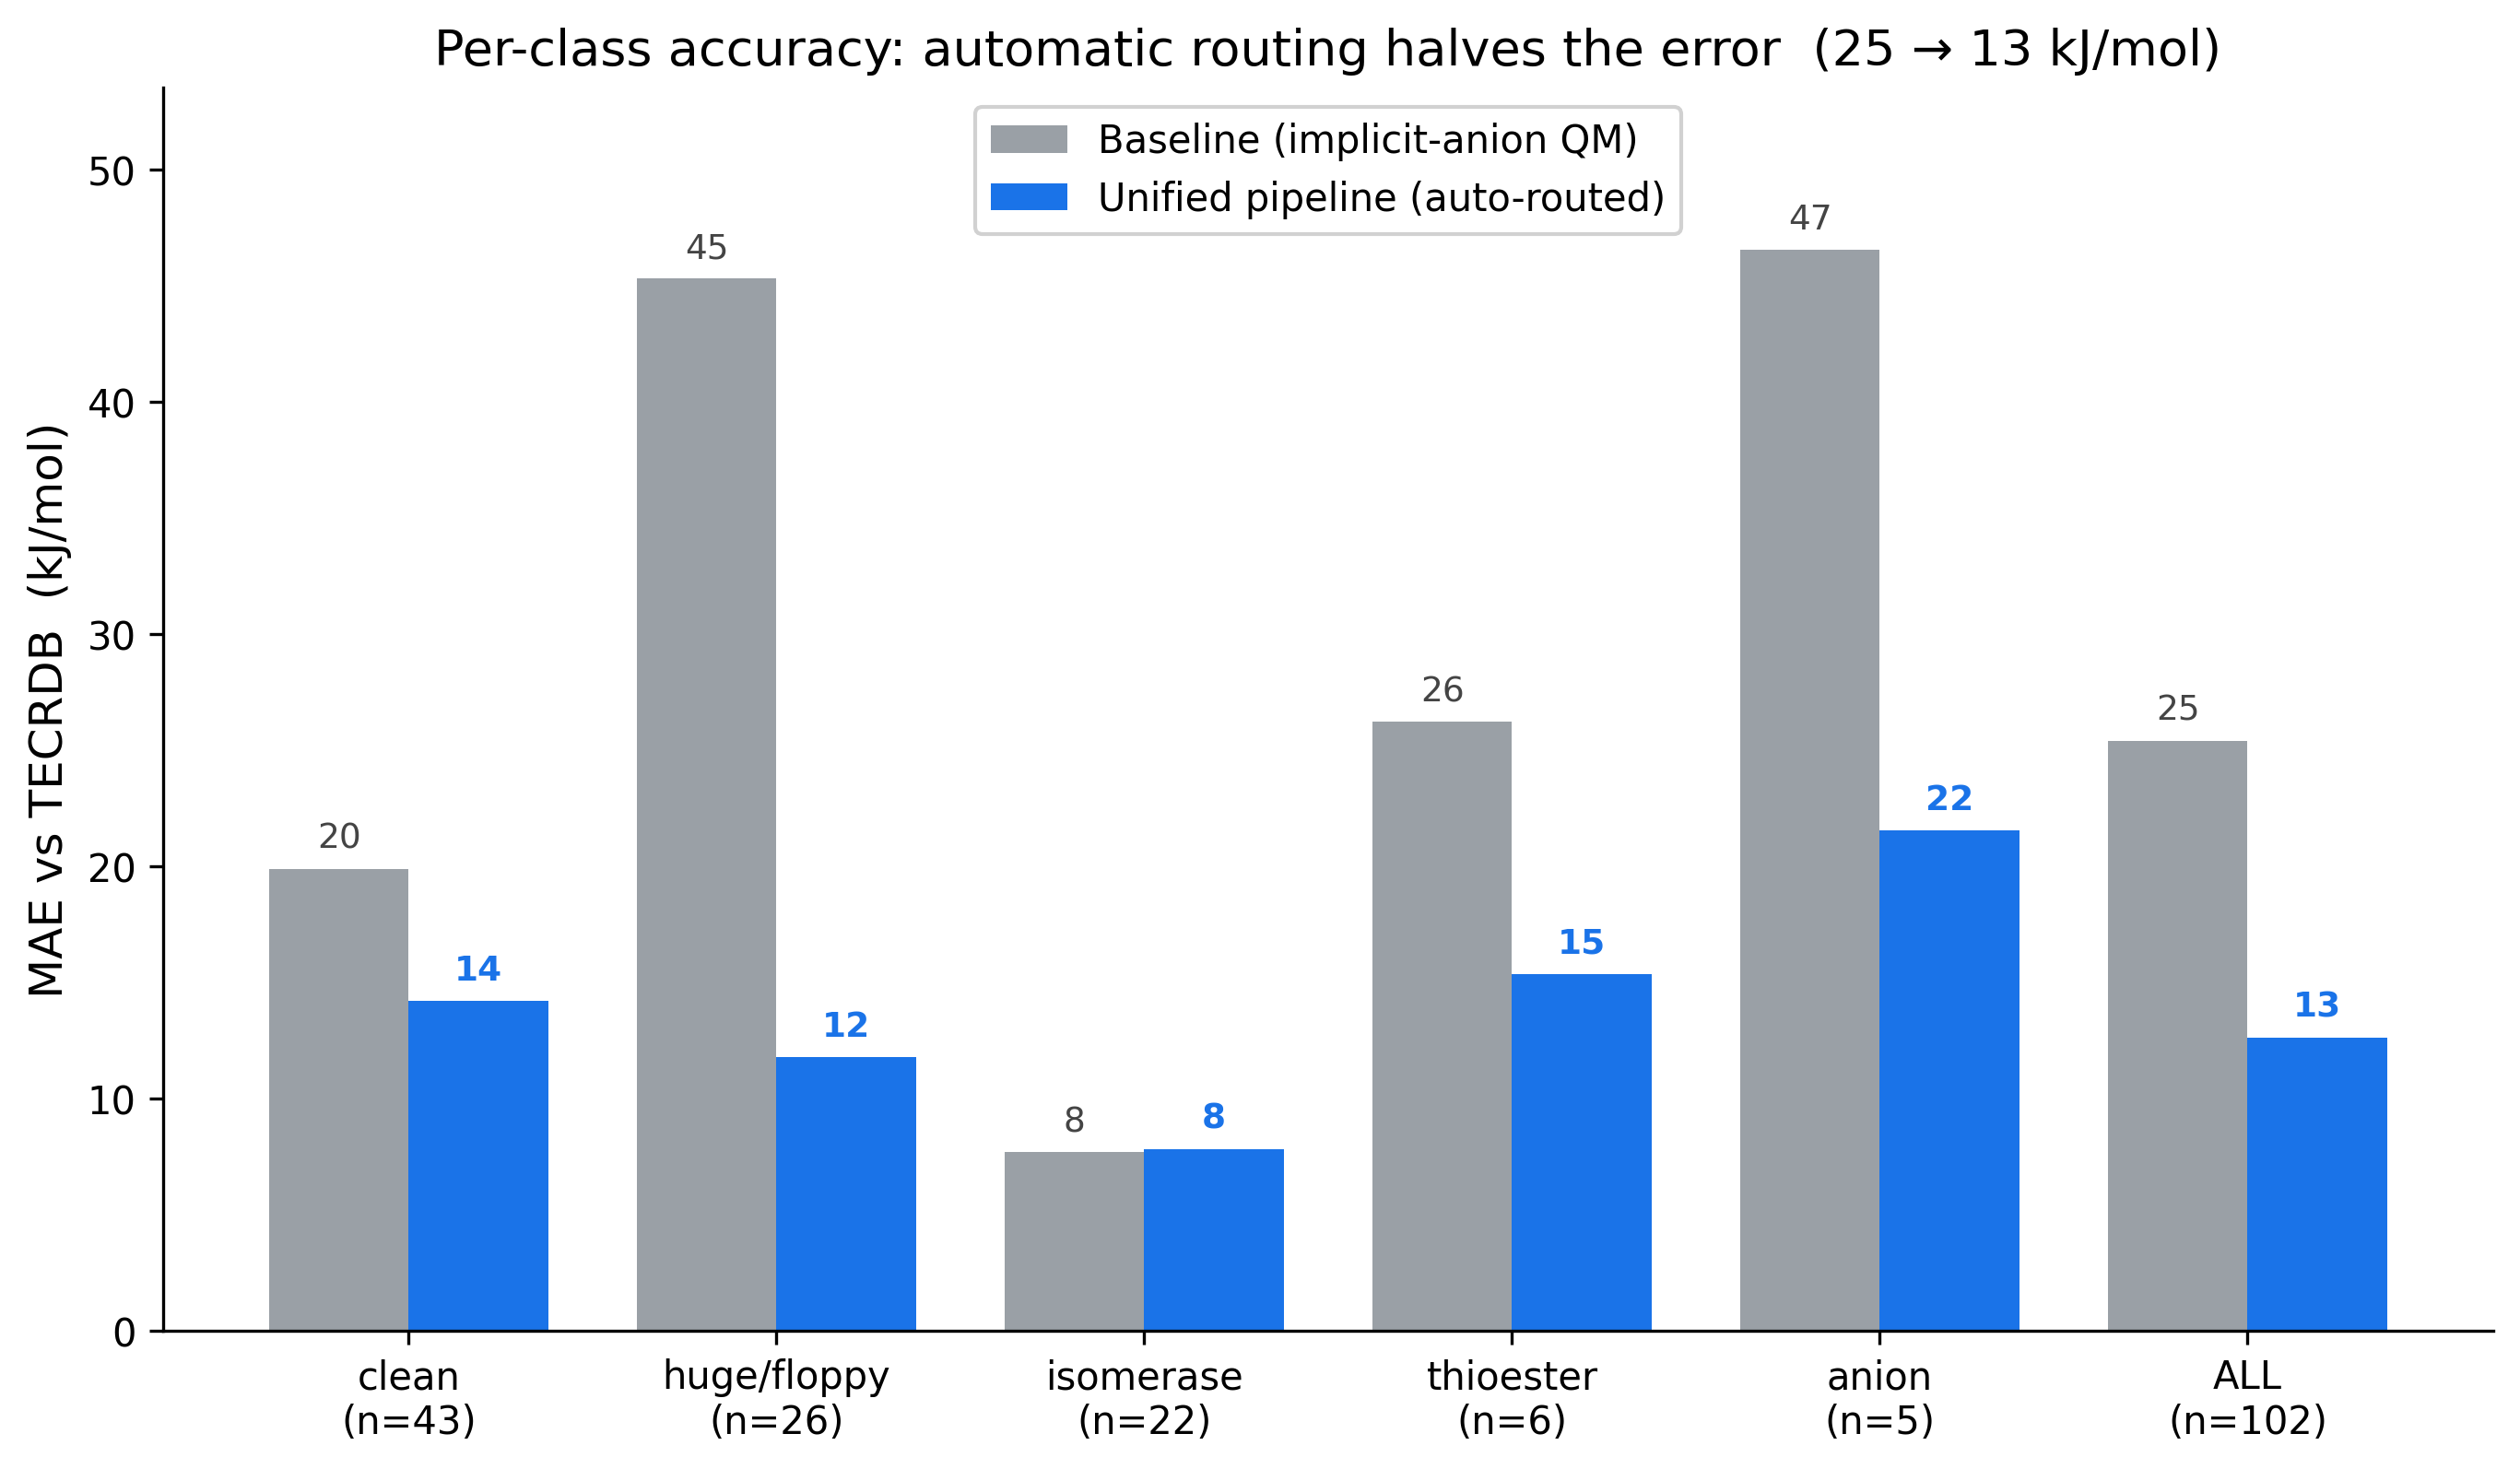
\includegraphics[width=0.82\textwidth]{deck_per_class_mae.png}
  \\[0.2em]
  {\footnotesize Matched subset, 117 processed so far. \emph{huge/floppy} $47\to18$;
  \emph{anion} (pure phosphoryl) $11\to\mathbf{6}$ --- pH-0 \emph{solves} it; \emph{glycosyl}
  (N-glycosidic transfer) $46\to27$ is the reference-method ceiling, not anion solvation;
  \emph{isomerase} unchanged (gated).}
\end{frame}

% ---- 11. RESULTS scatter ----------------------------------------------------------
\begin{frame}{Result: the high-error tail collapses}
  \centering
  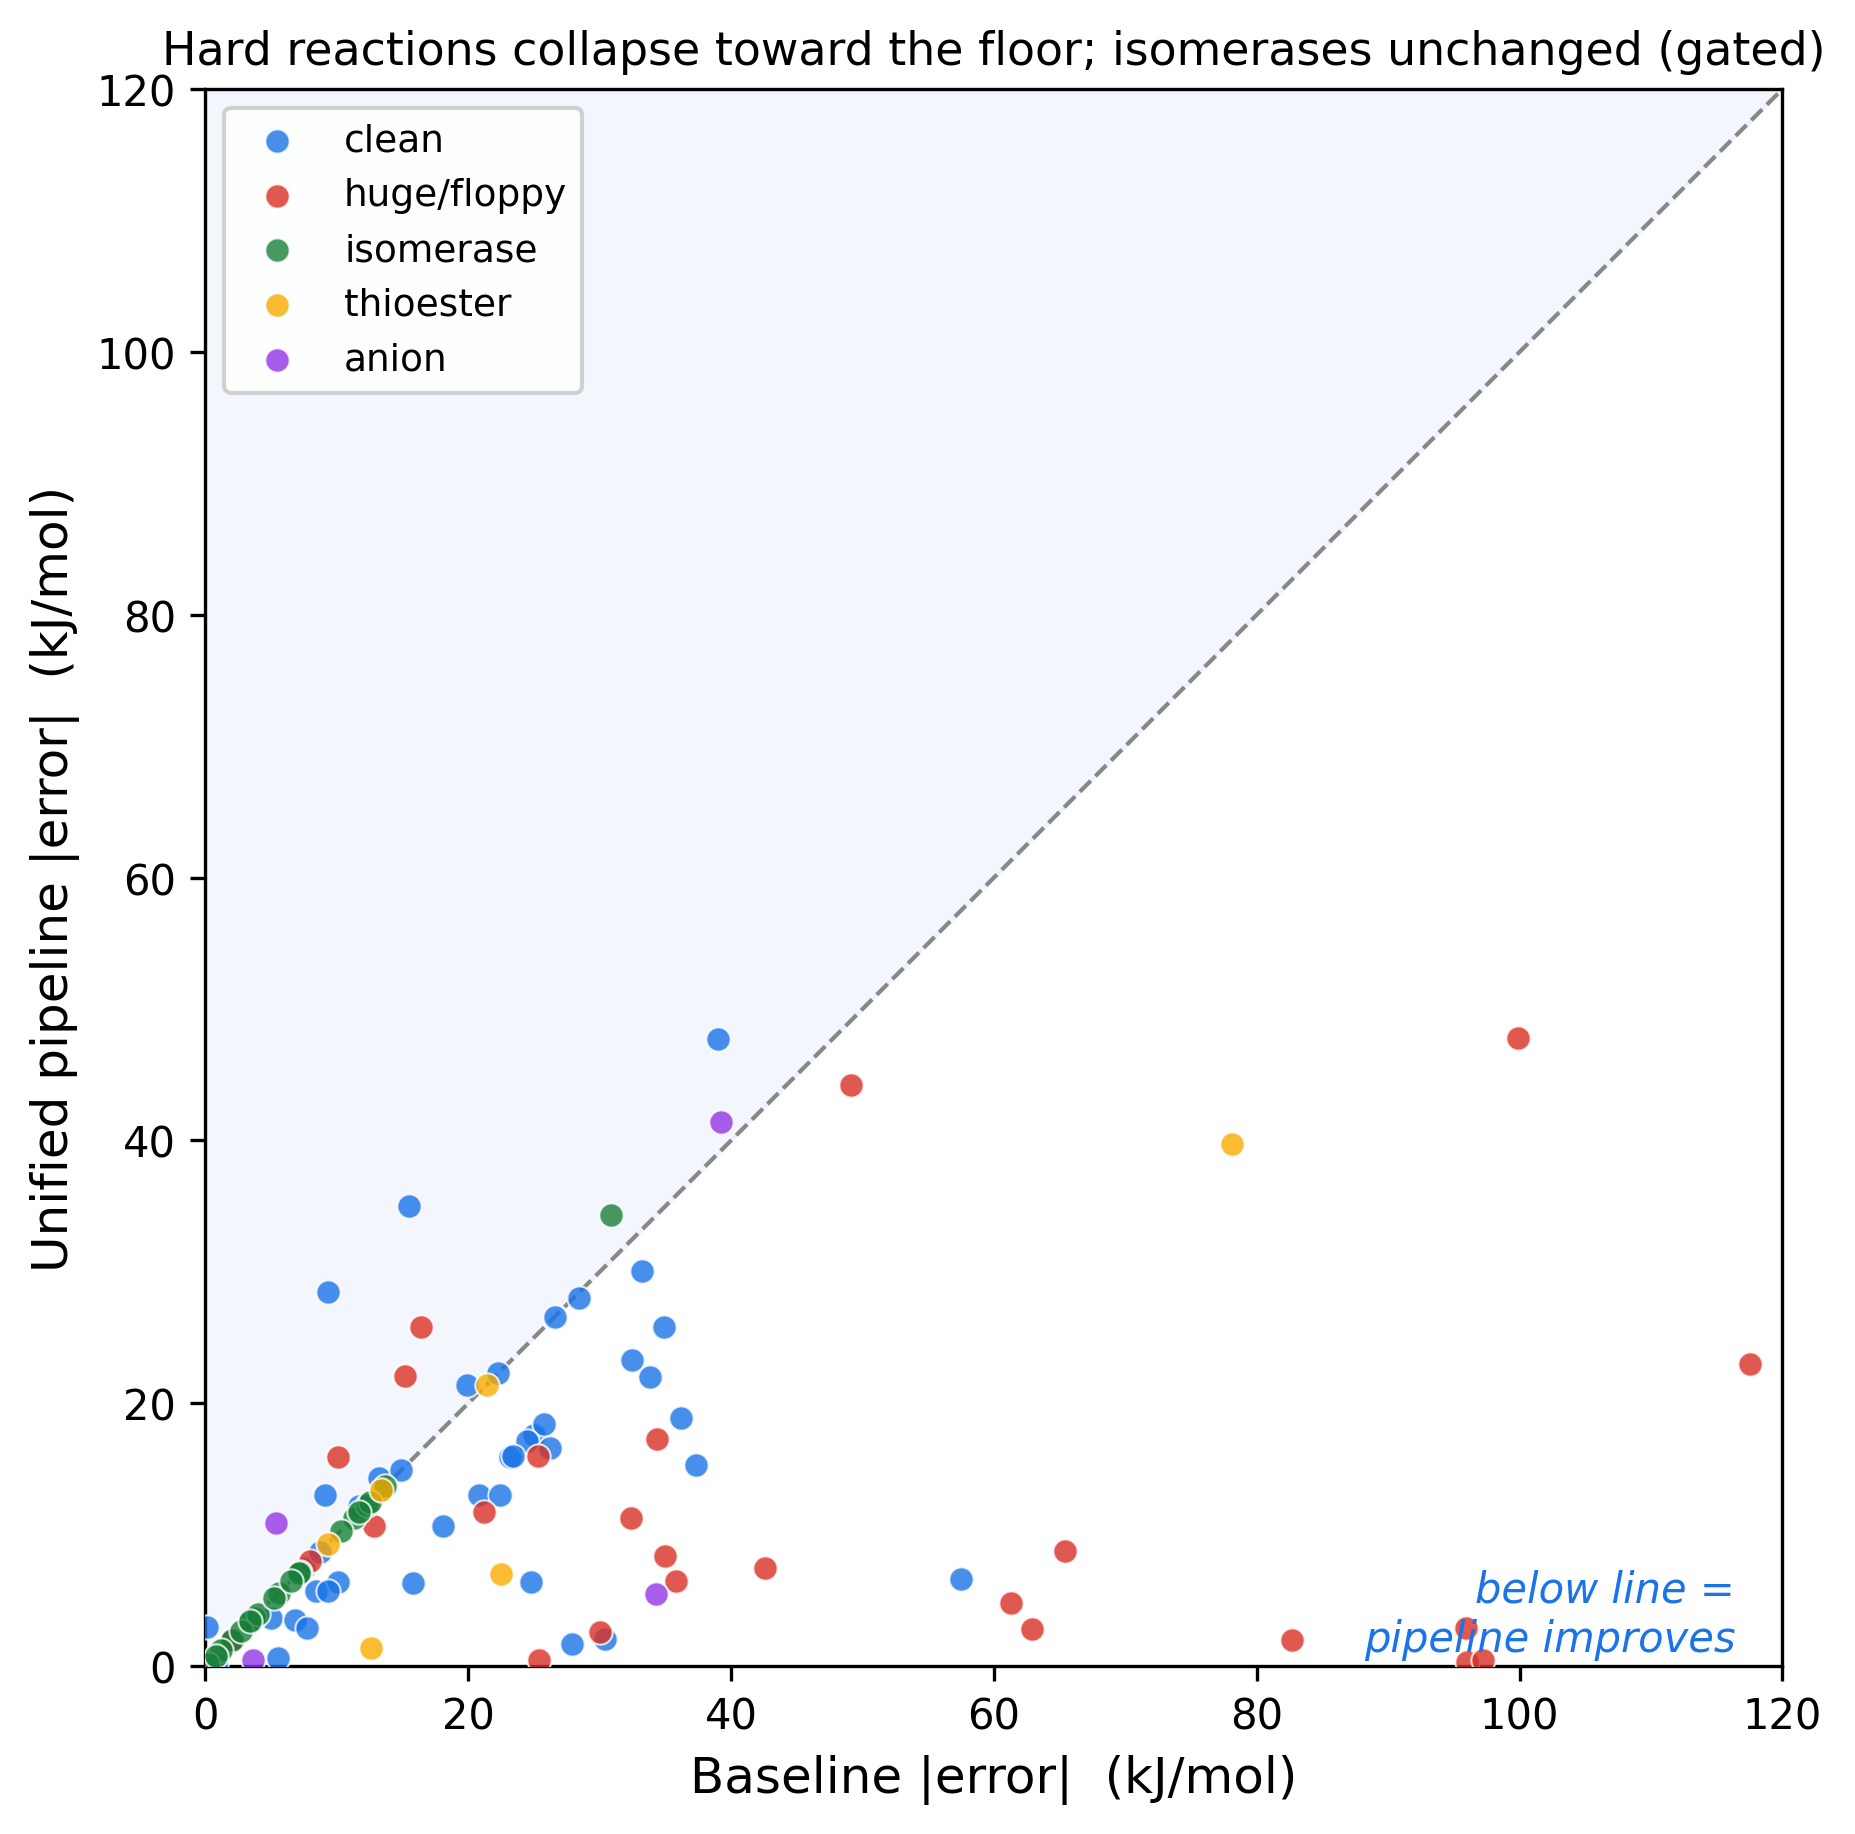
\includegraphics[height=0.78\textheight]{deck_before_after_scatter.png}
  \hfill
  \begin{minipage}{0.3\textwidth}\footnotesize
    Points below the diagonal improve. The worst baseline reactions ($80$–$118\kj$) drop under $25\kj$.
    Isomerases sit on the line — the gate leaves them alone.
  \end{minipage}
\end{frame}

% ---- 11b. HEAD-TO-HEAD vs dGPredictor ---------------------------------------------
\begin{frame}{Head-to-head where group-contribution struggles}
  \centering
  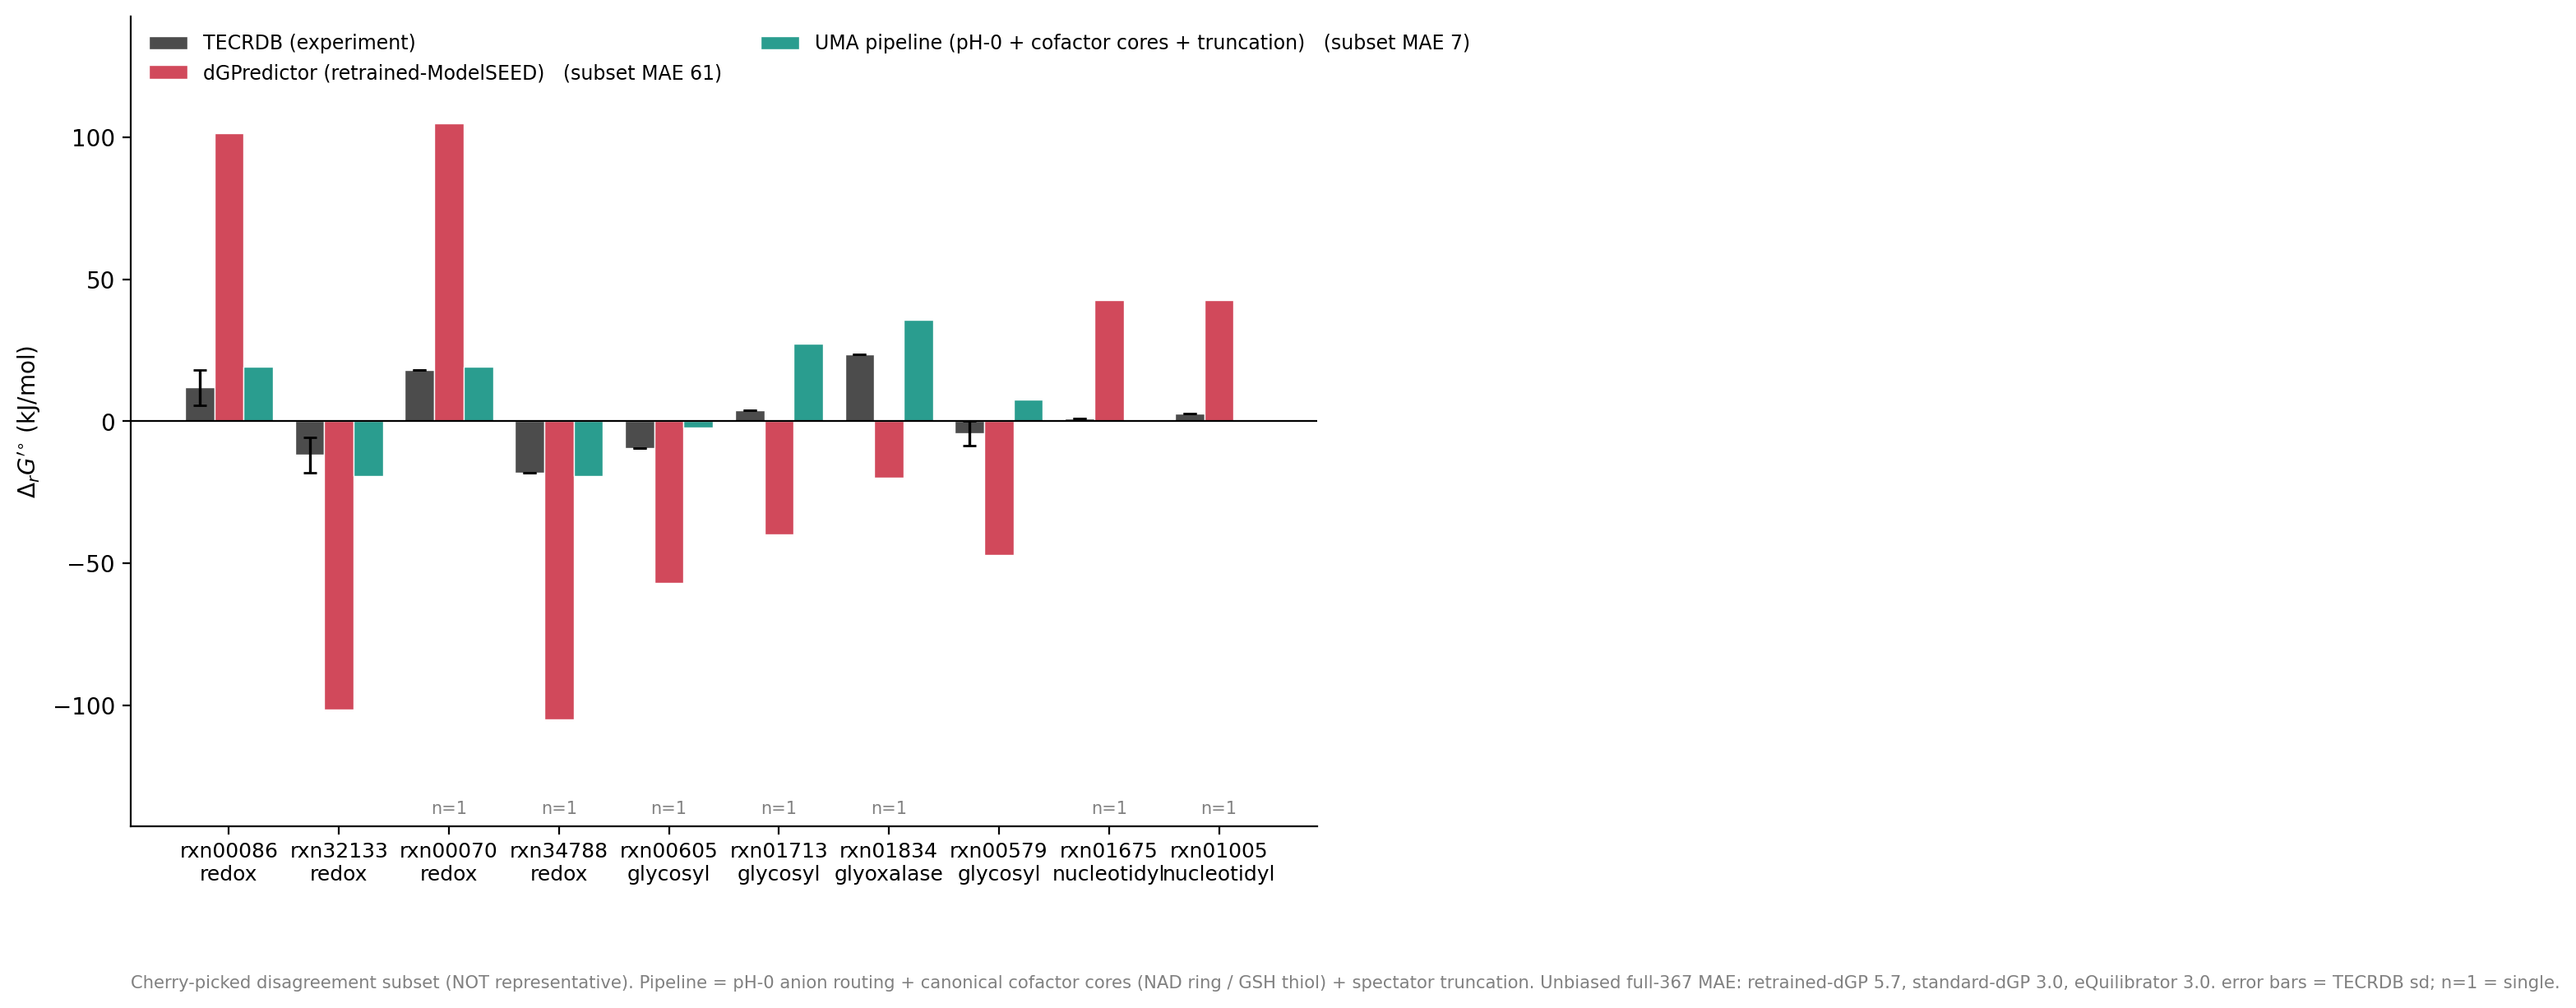
\includegraphics[width=0.92\textwidth]{deck_top10_comparison.png}
  \\[0.2em]
  {\footnotesize The 10 reactions where retrained-dGPredictor disagrees most with experiment
  (cherry-picked, \emph{not} representative). The QM pipeline (pH-0 $+$ ring-cofactor $+$ truncation)
  tracks experiment where the group method flies off by $80$–$100\kj$ --- the value is \textbf{coverage
  of the frontier}, not beating dGPredictor on its average (full-367 dGP $\approx$ 5.7).}
\end{frame}

% ---- 12. SCALE --------------------------------------------------------------------
\begin{frame}{From 367 benchmark reactions to the database}
  \begin{columns}[T]
    \begin{column}{0.55\textwidth}
      \begin{itemize}
        \item Validated on \textbf{TECRDB} (367 reactions with experimental $\Delta_r G$).
        \item Same code, one adapter \arw{} \textbf{20{,}802 ModelSEED reactions} runnable — no new flags.
        \item The router fires automatically: truncate \arw{} gated pH-0 \arw{} triage \arw{} QM \arw{} $\sigma$.
        \item \texttt{unified\_pipeline.py} is the single entry point; everything else is a library.
      \end{itemize}
    \end{column}
    \begin{column}{0.43\textwidth}
      \begin{block}{Coherent auto-router}
        \footnotesize No manual per-reaction decisions. Each reaction picks its own truncation
        radius, pH-0 eligibility, solvation model, and uncertainty from structure alone.
      \end{block}
      {\scriptsize Full-367 pH-0 sweep running across $\sim$37 GPUs; numbers here are the completed subset.}
    \end{column}
  \end{columns}
\end{frame}

% ---- 13. HONEST OPEN ITEMS --------------------------------------------------------
\begin{frame}{Honest open items}
  \begin{itemize}
    \item \textbf{Residual is scatter, not bias} \arw{} calibration won't shrink it; \emph{better referencing} will.
    Isodesmic / reference-reaction anchoring is the untapped multiplier.
    \item \textbf{Glycosyl electronic floor} is the \emph{reference method}, not UMA (DFT $\approx$ UMA $+0.7\kj$) — a genuine ceiling, flagged as reduced-confidence.
    \item \textbf{Mapping}: MCS vs RXNMapper — neither best alone (RXNMapper weak on phosphate, strong elsewhere); confidence-gated hybrid in progress.
    \item \textbf{Mg$^{2+}$}: subsumed by pH-0 on TECRDB; revisit only if a systematic-bias test demands explicit Mg.
    \item Finish the sweep \arw{} final aggregate $+$ per-class $\sigma$ calibration.
  \end{itemize}
\end{frame}

% ---- 14. SUMMARY ------------------------------------------------------------------
\begin{frame}{Summary}
  \begin{columns}[T]
    \begin{column}{0.62\textwidth}
      \begin{itemize}
        \item A \textbf{single automatic pipeline} scores metabolic $\Delta_r G$ from structure — no per-reaction tuning.
        \item \textbf{pH-0 routing} collapses the anion-solvation catastrophe; two structural gates keep it safe (isomerase, mass-balance).
        \item Matched-subset MAE \textbf{27 \arw{} 14\kj}; \emph{huge/floppy} \textbf{47 \arw{} 18}, pure-anion \textbf{11 \arw{} 6}.
        \item Scales to \textbf{20{,}802} ModelSEED reactions the group methods refuse.
      \end{itemize}
    \end{column}
    \begin{column}{0.36\textwidth}
      \begin{block}{Next}
        \footnotesize
        1. Finish sweep, calibrate $\sigma$.\\
        2. Isodesmic referencing.\\
        3. ModelSEED frontier demo (QM vs GCM).
      \end{block}
      \vspace{0.5em}
      {\scriptsize\color{brandgray} Method: UMA + xtb + Alberty transform. Parameter-free.}
    \end{column}
  \end{columns}
  \vfill
  \centering{\color{brandblue}\small Thank you --- questions?}
\end{frame}

\end{document}
